\documentclass[12pt,letterpaper]{report}

% =========================================================================
% Academic Formatting Requirements (Dr. Remudin Reshid Mekuria Standard)
% - Paper size: Letter (8.5 x 11 inches)
% - Margins: Top = 1.0 in, Bottom = 1.0 in, Right = 1.0 in, Left = 1.5 in (Binding)
% - Font: Times New Roman (12pt)
% - Spacing: Double-spaced text; tables, front matter, and references single-spaced
% - Alignment: Left-aligned (ragged right) with 0.5-inch paragraph indentation
% - Pagination: Prefatory = Roman numerals (bottom centered)
%               Main body = Arabic numerals (upper right corner)
% - Structure: Chapter I (Introduction), Chapter II (Review of Related Literature),
%              Chapter III (Conceptual Framework & Methodology), References, Appendixes
% =========================================================================

\usepackage[letterpaper, top=1.0in, bottom=1.0in, right=1.0in, left=1.5in]{geometry}
\usepackage{mathptmx} % Times New Roman font
\usepackage[T1]{fontenc}
\usepackage[utf8]{inputenc}
\usepackage{setspace}
\usepackage{ragged2e} % For left alignment with paragraph indents
\usepackage{amsmath,amssymb,amsfonts}
\usepackage{booktabs}
\usepackage{tabularx}
\usepackage{graphicx}
\usepackage{caption}
\usepackage{subcaption}
\usepackage{enumitem}
\usepackage{fancyhdr}
\usepackage{titlesec}
\usepackage{url}
\usepackage{hyperref}

% --- Paragraph and Indentation Settings (Slide 33) ---
\setlength{\RaggedRightParindent}{0.5in}
\setlength{\parindent}{0.5in}
\RaggedRight

% --- Double Spacing (Slide 32) ---
\doublespacing

% --- Table and Caption Formatting ---
\captionsetup{font={small,stretch=1.1}, labelfont=bf}

% --- Hyperlink Setup ---
\hypersetup{
    colorlinks=true,
    linkcolor=black,
    citecolor=black,
    urlcolor=blue!70!black
}

% --- Header and Footer / Pagination Setup (Slide 32) ---
\fancypagestyle{prefatory}{
    \fancyhf{}
    \fancyfoot[C]{\thepage} % Bottom centered small Roman numerals
    \renewcommand{\headrulewidth}{0pt}
}

\fancypagestyle{mainbody}{
    \fancyhf{}
    \fancyhead[R]{\thepage} % Upper right corner Arabic numerals
    \renewcommand{\headrulewidth}{0pt}
}

% --- Chapter Title Formatting (Slide 31) ---
\titleformat{\chapter}[display]
  {\normalfont\bfseries\centering}
  {\MakeUppercase{\chaptertitlename\ \thechapter}}
  {0.4em}
  {\large\MakeUppercase}
\titlespacing*{\chapter}{0pt}{0pt}{1.2em}

\titleformat{\section}
  {\normalfont\bfseries\normalsize}
  {\thesection}{1em}{}
\titlespacing*{\section}{0pt}{0.8em}{0.4em}

\titleformat{\subsection}
  {\normalfont\bfseries\small}
  {\thesubsection}{1em}{}
\titlespacing*{\subsection}{0pt}{0.6em}{0.3em}

% =========================================================================
\begin{document}

% -------------------------------------------------------------------------
% 1. TITLE PAGE (Slide 31 & 35: Unnumbered)
% -------------------------------------------------------------------------
\begin{titlepage}
\begin{center}
    \begin{singlespace}
        \textbf{\large ACADEMIC INSTITUTION / UNIVERSITY}\\
        \textbf{\large DEPARTMENT OF COMPUTER SCIENCE AND DATA SCIENCE}\\[2.0cm]

        \textbf{\Large EDUANALYTICS-KG: A 20-YEAR SPATIO-TEMPORAL MACHINE LEARNING AND ECONOMETRIC FRAMEWORK FOR ANALYZING REGIONAL DISPARITIES IN KYRGYZSTAN'S NATIONAL STANDARDIZED TESTING (ORT 2006--2025)}\\[1.8cm]

        \textit{A Master's Thesis Proposal (Second Draft / Revised Working Proposal)}\\
        \textit{Submitted in Partial Fulfillment of the Requirements}\\
        \textit{for the Degree of Master of Science in Data Science}\\[1.8cm]

        \textbf{Candidates / Authors:}\\
        Aidin Turdukulov\\
        Argen Kulzhanov\\[1.0cm]

        \textbf{Thesis Adviser:}\\
        Dr. Research Supervisor / Thesis Consultant\\[1.8cm]

        Bishkek, Kyrgyz Republic\\
        October 2026
    \end{singlespace}
\end{center}
\end{titlepage}

% -------------------------------------------------------------------------
% PREFATORY PAGES (Slide 32: Roman numerals, centered at bottom)
% -------------------------------------------------------------------------
\pagestyle{prefatory}
\pagenumbering{roman}
\setcounter{page}{2}

% --- Abstract (Slide 32 & Academic Thesis Proposal Standard) ---
\chapter*{Abstract}
\addcontentsline{toc}{chapter}{Abstract}

This master's thesis proposal presents the research design and methodological architecture of \textbf{EduAnalytics-KG}, an integrated spatial econometric and machine learning framework designed to investigate the structural determinants of long-term regional performance disparities in the Kyrgyz Republic's National Standardized Testing (\textit{Общереспубликанское тестирование}, ORT). Spanning two decades (2006--2025), the study constructs a comprehensive six-tier data ecosystem comprising $12,320$ harmonized observations across micro, network, meso, and macro dimensions: (i) an unbroken 20-year administrative district census panel ($N = 889$ district-years expanded to 38 structural features); (ii) the complete national registry of $2,386$ secondary schools from the Education Management Information System (EMIS / \textit{ИСУО}); (iii) an origin-destination academic mobility network tracking $6,575$ district-to-university grant flows ($51,646$ students across 37 higher education institutions); (iv) a 20-year multi-subject performance panel ($N = 243$ records across 10 disciplines and testing languages); (v) a 20-year regional macroeconomic and cohort series from the National Statistical Committee (NatStatCom, $N = 180$); and (vi) a longitudinal gender disparity series ($N = 14$ years).

Standardized testing in Kyrgyzstan governs university matriculation and state-funded scholarship distribution. Despite a statutory affirmative action quota system established in 2002, substantial spatial stratification persists between the capital city of Bishkek (mean scores $>133$ points) and remote mountainous perimeters (averaging $\sim 110$ points). Current policy planning is limited by isolated annual reporting and a lack of predictive modeling. This research formulates a dual analytical pipeline: (i) an econometric Two-Way Fixed Effects (TWFE) and Spatial Autoregressive (SAR) baseline measuring structural elasticities across pupil-teacher ratios, poverty headcount rates, and teacher qualifications; and (ii) a supervised Gradient Boosted Decision Tree architecture (CatBoost) evaluated under spatial block cross-validation and out-of-time temporal hold-out testing (2006--2021 train, 2022--2025 test). Model predictions are decomposed via TreeSHAP (SHapley Additive exPlanations) to uncover non-linear institutional tipping points. Finally, an interactive Decision Support System (DSS) prototype is specified to simulate ``What-If'' counterfactual budget allocations. Preliminary exploratory data analysis validates data ingestion accuracy ($R^2 = 0.74$ on out-of-time test sets), establishing the empirical feasibility of the proposed investigation.

\vspace{0.8cm}
\begin{singlespace}
\noindent\textbf{Keywords:} Educational Data Mining, Standardized Testing, ORT, Spatial Econometrics, CatBoost, Explainable AI, TreeSHAP, Kyrgyzstan, Regional Disparities, Decision Support System.
\end{singlespace}

\newpage

% --- Table of Contents ---
\begin{singlespace}
\tableofcontents
\newpage

% --- Consolidated List of Tables & Figures (Slide 35) ---
\listoftables
\vspace{1.5cm}
\listoffigures
\newpage

% --- List of Abbreviations (Slide 35) ---
\chapter*{List of Abbreviations}
\addcontentsline{toc}{chapter}{List of Abbreviations}
\begin{tabularx}{\textwidth}{l X}
\textbf{ADM1} & First-Level Administrative Subdivisions (Provinces / Oblasts) \\
\textbf{ADM2} & Second-Level Administrative Subdivisions (Districts / Rayons) \\
\textbf{CatBoost} & Categorical Boosting (Gradient Boosted Decision Trees) \\
\textbf{CEAMO} & Center for Educational Assessment and Methods (\textit{ЦООМО}) \\
\textbf{CF} & Conceptual Framework \\
\textbf{DiD} & Difference-in-Differences \\
\textbf{DSS} & Decision Support System \\
\textbf{EDM} & Educational Data Mining \\
\textbf{EMIS} & Education Management Information System (\textit{ИСУО}) \\
\textbf{ENEM} & \textit{Exame Nacional do Ensino Médio} (National High School Exam, Brazil) \\
\textbf{IRT} & Item Response Theory \\
\textbf{KGS} & Kyrgyz Som (National Currency of the Kyrgyz Republic) \\
\textbf{MAE} & Mean Absolute Error \\
\textbf{MOES} & Ministry of Education and Science of the Kyrgyz Republic \\
\textbf{NatStatCom} & National Statistical Committee of the Kyrgyz Republic \\
\textbf{OLS} & Ordinary Least Squares \\
\textbf{ORT} & National Scholarship Testing (\textit{Общереспубликанское тестирование}) \\
\textbf{PISA} & Programme for International Student Assessment (OECD) \\
\textbf{RMSE} & Root Mean Squared Error \\
\textbf{RRL} & Review of Related Literature \\
\textbf{SAR} & Spatial Autoregressive Model \\
\textbf{SEM} & Spatial Error Model \\
\textbf{SES} & Socioeconomic Status \\
\textbf{SHAP} & Shapley Additive Explanations \\
\textbf{SOATO} & State Classifier of Administrative-Territorial Units (\textit{СОАТО}) \\
\textbf{TWFE} & Two-Way Fixed Effects Panel Model \\
\textbf{XAI} & Explainable Artificial Intelligence \\
\end{tabularx}
\end{singlespace}

\newpage

% -------------------------------------------------------------------------
% MAIN BODY (Slide 32: Arabic numerals, upper right corner)
% -------------------------------------------------------------------------
\pagestyle{mainbody}
\pagenumbering{arabic}
\setcounter{page}{1}

% =========================================================================
\chapter{Introduction}
\label{chap:intro}
% =========================================================================

\section{Essence of the Study}
This master's thesis proposal investigates the structural, socioeconomic, and institutional determinants of regional disparities in standardized university entrance examinations across the Kyrgyz Republic. Specifically, the proposed study develops \textbf{EduAnalytics-KG}, an integrated machine learning and spatial econometric framework applied to a newly constructed 20-year longitudinal panel dataset covering all 52 administrative districts and municipalities from 2006 to 2025. Standardized examination results serve as the primary meritocratic gateway to tertiary education and social mobility in developing transition economies. By coupling administrative test micro-aggregates with district-level macroeconomic and institutional features, this research models educational production functions, uncovers non-linear structural thresholds, and operationalizes an interactive Decision Support System (DSS) prototype for evidence-based resource allocation.

\section{Rationale and Problem Context}
Following national independence in 1991, higher education admissions in Central Asia were severely compromised by institutional corruption, non-standardized grading, and acute rural-urban inequities. In 2002, the Ministry of Education and Science of the Kyrgyz Republic (MOES), supported by USAID, established the National Scholarship Testing (\textit{Общереспубликанское тестирование}, ORT), administered by the independent Center for Educational Assessment and Methods (CEAMO / \textit{ЦООМО}) (Drummond \& DeYoung, 2006).

The examination is a high-stakes standardized gatekeeper: achieving a statutory baseline (historically 110 points on a 245-point scale) is required for university matriculation, while top percentiles compete for approximately 5,000 full-tuition state scholarships (\textit{бюджетные гранты}). To protect disadvantaged applicants, the government introduced a three-tiered affirmative action quota dividing examinees into: (i) Capital schools (Bishkek); (ii) Regional centers and small towns; and (iii) Rural and high-altitude schools.

Despite two decades of quota administration, severe spatial divergence persists. The capital city of Bishkek consistently records average scores above 133 points, whereas peripheral districts in Batken, Naryn, and mountainous Osh regularly average near the 110-point threshold, with qualification pass rates dipping below 50\%. Current educational planning remains largely retrospective, relying on disconnected annual cross-sectional reports that cannot measure the marginal return of public investments or teacher incentive policies.

\section{Research Purposes and Primary Objectives}
The central objective of this research is to advance educational administration in Kyrgyzstan from descriptive retrospective reporting into a predictive, evidence-based planning paradigm. The specific objectives to be carried out are:
\begin{enumerate}[noitemsep,topsep=2pt,parsep=0pt]
    \item \textbf{Data Ingestion \& Harmonization:} Complete, clean, and standardize the 20-year census panel dataset (2006--2025) of ORT metrics across all 52 administrative units, harmonized with official NatStatCom indicators.
    \item \textbf{Econometric Baseline Formulation:} Estimate Two-Way Fixed Effects (TWFE) and Spatial Autoregressive (SAR) specifications measuring the elasticity of test performance with respect to pupil-teacher ratios, poverty rates, wages, and teacher credentials.
    \item \textbf{Machine Learning Benchmarking:} Train and validate regularized tree-based ensembles (CatBoost, LightGBM) under spatial block cross-validation and out-of-time temporal hold-out evaluation (Train: 2006--2021; Test: 2022--2025).
    \item \textbf{Explainable AI and Threshold Discovery:} Apply TreeSHAP to identify structural inflection points (e.g., classroom congestion tipping points) that linear specifications conceal.
    \item \textbf{Decision Support System Prototype:} Formulate a counterfactual simulation module enabling educational authorities to forecast the impact of targeted fiscal interventions.
\end{enumerate}

\section{Significance and Target Readership}
This research provides direct empirical and computational value to three primary audiences: (i) \textbf{Policymakers} at MOES, the Ministry of Finance, and CEAMO seeking empirical justification for targeted school construction and teacher hardship allowances; (ii) \textbf{Development Partners} (World Bank, UNICEF, ADB) requiring rigorous impact assessment methodologies; and (iii) \textbf{Scholars} in educational data mining and development economics studying post-Soviet transition economies.

\section{Central Research Questions and Hypotheses}
The investigation will formally address three core research questions:
\begin{quote}
\textit{RQ1: How have spatial disparities evolved across Kyrgyzstan's 52 districts over the 2006--2025 period, and does empirical evidence indicate regional convergence or persistent divergence?}

\textit{RQ2: What are the marginal elasticities of pedagogical and socioeconomic features, and do non-linear structural thresholds govern test score sensitivity?}

\textit{RQ3: Can regularized machine learning models generalize across time and geography to enable reliable counterfactual policy simulations?}
\end{quote}

The research formally tests three primary hypotheses:
\begin{itemize}[noitemsep,topsep=2pt,parsep=0pt]
    \item \textbf{Hypothesis 1 ($H_1$):} Pupil-teacher ratios exhibit a critical non-linear tipping point ($>18:1$) beyond which academic performance deteriorates at an accelerating rate.
    \item \textbf{Hypothesis 2 ($H_2$):} Marginal returns on teacher qualifications and classroom decongestion significantly outweigh nominal salary subsidies in remote high-altitude districts.
    \item \textbf{Hypothesis 3 ($H_3$):} District-level performance demonstrates significant positive spatial autocorrelation ($\rho > 0$), necessitating spatial econometric controls.
\end{itemize}

\section{Logic Chain of the Research}
The operational logic chain proceeds systematically:
\begin{equation*}
    \text{Data Ingestion} \longrightarrow \text{Feature Fusion} \longrightarrow \text{TWFE / SAR Baseline} \longrightarrow \text{CatBoost / TreeSHAP} \longrightarrow \text{What-If Simulation}
\end{equation*}


% =========================================================================
\chapter{Review of Related Literature}
\label{chap:rrl}
% =========================================================================

\section{Theoretical Foundations: The Educational Production Function}
The theoretical foundation of this study is rooted in the Educational Production Function framework formalized by Coleman et al. (1966) and Hanushek (1979, 2006). Under this paradigm, student academic achievement ($Y$) is modeled as a functional output of cumulative inputs:
\begin{equation}
    Y_{it} = f(\mathbf{F}_{it}, \mathbf{S}_{it}, \mathbf{P}_{it}, \mathbf{C}_{it})
\end{equation}
where $\mathbf{F}_{it}$ denotes family socioeconomic endowment, $\mathbf{S}_{it}$ represents school inputs (pupil-teacher ratios, teacher credentials), $\mathbf{P}_{it}$ reflects peer group attributes, and $\mathbf{C}_{it}$ represents broader community and geographic characteristics. While Hanushek (1986) suggested weak correlations between marginal school funding and outcomes in developed economies, subsequent empirical studies (Card \& Krueger, 1992; Chetty et al., 2014) demonstrated that classroom scale and teacher quality exert substantial returns in resource-constrained environments.

\section{International Standardized Testing Analytics}
To contextualize Kyrgyzstan's assessment landscape, Table~\ref{tab:comparison_lit} synthesizes major international standardized examination analytics.

\begin{table}[htbp]
\centering
\begin{singlespace}
\small
\caption{Comparative synthesis of international standardized testing analytics.}
\label{tab:comparison_lit}
\begin{tabularx}{\textwidth}{l p{2.6cm} p{3.2cm} X}
\toprule
\textbf{Examination} & \textbf{Jurisdiction} & \textbf{Methodology} & \textbf{Key Empirical Findings} \\
\midrule
\textbf{SAT / ACT} & United States & OLS, Regression Discontinuity & Socioeconomic status accounts for $>40\%$ variance; non-linear class size effects (Chetty et al., 2014). \\
\textbf{ENEM} & Brazil & Random Forests, XGBoost & Substantial public-private and regional divide; high predictive power for higher education access (Marteleto et al., 2016). \\
\textbf{Saber 11} & Colombia & Deep Neural Networks, Spatial DiD & Conflict exposure and municipal poverty generate persistent regional score deficits (Saenz et al., 2020). \\
\textbf{PISA (OECD)} & Central Asia Region & Multi-Level Hierarchical Linear Models & Identifies acute rural-urban literacy gaps; Central Asian scores consistently lag OECD medians by $>1.5$ standard deviations. \\
\midrule
\textbf{ORT (This Study)} & \textbf{Kyrgyz Republic} & \textbf{Multi-Tier Ecosystem (N=12,320) + TWFE/SAR + CatBoost/TreeSHAP} & \textbf{First census-scale spatio-temporal framework linking 20-year testing, 2,386 schools, 6,575 HEI flows, and counterfactual DSS.} \\
\bottomrule
\end{tabularx}
\end{singlespace}
\end{table}

\section{Spatial Econometrics and Regional Inequality}
Educational opportunities exhibit strong spatial dependency. Following Tobler's First Law of Geography, neighboring administrative districts share labor pools, pedagogical practices, and economic shocks. Standard Ordinary Least Squares (OLS) estimation under spatial dependency yields biased and inconsistent estimates (Anselin, 1988). Incorporating a row-standardized spatial contiguity weight matrix $\mathbf{W}$ allows estimation of Spatial Autoregressive (SAR) and Spatial Error (SEM) specifications to separate endogenous spatial spillovers from unobserved spatial error correlations.

\section{Machine Learning and Explainability in Educational Policy}
Recent advances in Gradient Boosted Decision Trees (GBDT)—notably CatBoost (Prokhorenkova et al., 2018)—have revolutionized tabular predictive modeling by handling complex multi-way interaction effects and categorical features without target leakage. To resolve the ``black box'' limitation, TreeSHAP (Lundberg \& Lee, 2017) provides an axiomatic game-theoretic decomposition of individual feature contributions, enabling the discovery of localized non-linear thresholds critical for evidence-based policy.

\section{Critical Gaps in the Literature}
Table~\ref{tab:gaps} details the fundamental literature gaps that this proposed study is designed to bridge.

\begin{table}[htbp]
\centering
\begin{singlespace}
\small
\caption{Identified literature gaps and methodological solutions in EduAnalytics-KG.}
\label{tab:gaps}
\begin{tabularx}{\textwidth}{l p{4.5cm} X}
\toprule
\textbf{Dimension} & \textbf{Status of Existing Literature} & \textbf{EduAnalytics-KG Resolution} \\
\midrule
Temporal Horizon & Single-year cross-sectional surveys ($N < 500$). & Complete 20-year census panel ($2006\text{--}2025$, $N=889$). \\
Spatial Modeling & Non-spatial descriptive provincial aggregates. & District-level spatial weight matrices ($\mathbf{W}$) and SAR modeling. \\
Functional Form & Rigid parametric linear assumptions (OLS). & Non-parametric CatBoost GBDT capturing non-linear thresholds. \\
Policy Translation & Generic qualitative policy discussions. & Interactive counterfactual What-If simulation engine. \\
\bottomrule
\end{tabularx}
\end{singlespace}
\end{table}


% =========================================================================
\chapter{Conceptual Framework and Research Methodology}
\label{chap:methodology}
% =========================================================================

\section{Conceptual Framework}
The conceptual framework structuring this research is illustrated in Figure~\ref{fig:conceptual_framework}. The model posits that district examination performance ($Y$) is driven by three interconnected input domains: (i) Institutional and pedagogical resources; (ii) Territorial socioeconomic conditions; and (iii) Geographic topography.

\begin{figure}[htbp]
\centering
\begin{singlespace}
\fbox{
\begin{minipage}{0.92\textwidth}
\centering \small
\textbf{STRUCTURAL INPUTS ($X$): 52 TERRITORIES (2006--2025, N = 889)}\\[0.3em]
\begin{tabularx}{\textwidth}{X | X | X}
\textbf{Pedagogical Factors} & \textbf{Socioeconomic Context} & \textbf{Geographic Topography} \\
Pupil-Teacher Ratio (PTR) & Poverty Headcount Rate (\%) & High-Altitude Flag ($\ge 1800$m) \\
Teachers Tertiary Ed. (\%) & Avg. Monthly Wage (KGS) & Rural Population Share (\%) \\
Candidate Cohort Volume & Industrial Output Volume & Boundary Isolation Index \\
\end{tabularx}
\\[0.3em]
$\Big\downarrow$ \textit{Dual Econometric and Machine Learning Engine} \\[0.3em]
\begin{tabularx}{\textwidth}{X | X}
\textbf{Econometric Branch: TWFE \& SAR} & \textbf{Machine Learning Branch: CatBoost GBDT} \\
$Y_{it} = \rho \mathbf{W} Y_{it} + \mathbf{X}_{it}' \boldsymbol{\beta} + \alpha_i + \lambda_t + \varepsilon_{it}$ & Spatial Block Cross-Validation \\
Controls unobserved time-invariant heterogeneity & Non-linear interactions \& threshold discovery \\
\end{tabularx}
\\[0.3em]
$\Big\downarrow$ \textit{Explainable AI Decomposition (TreeSHAP)} \\[0.3em]
\textbf{POLICY ARTIFACTS: Overcrowding Thresholds ($>18:1$) + Interactive Counterfactual DSS Engine}
\end{minipage}
}
\caption{Conceptual framework of the EduAnalytics-KG research architecture.}
\label{fig:conceptual_framework}
\end{singlespace}
\end{figure}

\section{Research Design and Multi-Tier Data Architecture}
This study adopts a \textbf{quantitative, multi-resolution longitudinal research design} combining supervised machine learning, spatial econometrics, and network flow analysis. Because CEAMO and the Ministry of Education explicitly refrain from publishing raw school-by-school average ORT rankings to prevent rural school stigmatization, demoralization, and ``teaching to the test'' distortions (CEAMO Annual Report, 2025, p.~22), this research constructs a six-tier harmonized data architecture totaling $12,320$ records (Table~\ref{tab:data_ecosystem}).

\begin{table}[htbp]
\centering
\begin{singlespace}
\small
\caption{Multi-tier data ecosystem constructed for EduAnalytics-KG ($12,320$ total observations).}
\label{tab:data_ecosystem}
\begin{tabularx}{\textwidth}{l l c X}
\toprule
\textbf{Data Tier} & \textbf{Spatial / Unit Resolution} & \textbf{Records ($N$)} & \textbf{Primary Variables and Official Source} \\
\midrule
Tier 1: School Registry & Micro (Individual School) & $2,386$ & OKPO ID, ownership (public/private), gymnasium/lyceum status, SOATO district link (EMIS / \texttt{data.gov.kg}). \\
Tier 2: Mobility Network & Network ($\text{Rayon} \to \text{University}$) & $6,575$ & Origin-destination grant flows ($51,646$ students across 37 HEIs, 2015--2025, CEAMO App.~VI). \\
Tier 3: Master Enriched Panel & Meso ($\text{District} \times \text{Year}$) & $889$ & Core 20-year census panel expanded to 38 features across 52 territories (2006--2025). \\
Tier 4: Subject Panel & Domain ($\text{Subject} \times \text{Language}$) & $243$ & 20-year performance across 10 STEM and Humanities tests by language (CEAMO App.~II). \\
Tier 5: Macro Cohort Matrix & Macro ($\text{Region} \times \text{Year}$) & $180$ & 11th-grade graduate cohorts, school counts, student bodies, and female teachers (NatStatCom). \\
Tier 6: Gender Gap Series & National ($\text{Gender} \times \text{Year}$) & $14$ & Female vs. male mean scores (+8.10 pt female advantage) and grant shares (60.94\% female). \\
\bottomrule
\end{tabularx}
\end{singlespace}
\end{table}

By linking the $2,386$ school records from the national EMIS registry to administrative districts, the framework computes exact structural school-network indicators—such as the district share of specialized gymnasiums and lyceums (\texttt{specialized\_schools\_share}) and private institutions (\texttt{private\_schools\_share})—thereby capturing institutional school quality without violating statutory privacy guidelines.

\section{Pilot Exploratory Data Analysis \& Descriptive Statistics}
Table~\ref{tab:eda_stats} provides baseline descriptive statistics calculated from the enriched 38-feature 20-year district census panel ($N = 889$), establishing empirical feasibility.

\begin{table}[htbp]
\centering
\begin{singlespace}
\small
\caption{Descriptive statistics of the enriched 20-year district panel dataset ($2006\text{--}2025$, $N = 889$, selected variables from 38 features).}
\label{tab:eda_stats}
\begin{tabularx}{\textwidth}{l c c c c X}
\toprule
\textbf{Variable Identifier} & \textbf{Mean} & \textbf{Std. Dev.} & \textbf{Min} & \textbf{Max} & \textbf{Description} \\
\midrule
\texttt{mean\_score} & $116.4$ & $6.82$ & $98.4$ & $142.2$ & Mean district ORT score [80--245]. \\
\texttt{pass\_rate\_pct} & $54.2\%$ & $12.4\%$ & $21.8\%$ & $88.6\%$ & Examinees exceeding 110-point cutoff. \\
\texttt{specialized\_schools\_share} & $14.2\%$ & $9.80\%$ & $0.0\%$ & $39.0\%$ & Share of gymnasiums/lyceums in district. \\
\texttt{private\_schools\_share} & $4.8\%$ & $8.15\%$ & $0.0\%$ & $34.1\%$ & Share of private schools in district. \\
\texttt{regional\_ort\_coverage} & $74.6\%$ & $14.2\%$ & $41.2\%$ & $100.0\%$ & Share of 11th-grade cohort taking ORT. \\
\texttt{pupil\_teacher\_ratio} & $16.8$ & $3.45$ & $9.2$ & $26.4$ & Ratio of enrolled pupils to teachers. \\
\texttt{teachers\_higher\_ed} & $86.4\%$ & $6.12\%$ & $68.1\%$ & $98.4\%$ & Instructors with university degrees. \\
\texttt{avg\_monthly\_salary} & $12,450$ & $8,120$ & $1,840$ & $48,200$ & Mean nominal monthly wage (KGS). \\
\texttt{poverty\_rate\_pct} & $28.4\%$ & $11.8\%$ & $8.2\%$ & $62.4\%$ & Share below national poverty line. \\
\texttt{rural\_population} & $68.2\%$ & $28.6\%$ & $0.0\%$ & $100.0\%$ & Rural residency proportion. \\
\bottomrule
\end{tabularx}
\end{singlespace}
\end{table}

\section{Analytical Methods and Model Specifications}
\subsection{Two-Way Fixed Effects (TWFE) and Spatial Autoregressive (SAR) Models}
The baseline econometric specification is formulated as:
\begin{equation}
    Y_{it} = \alpha_i + \lambda_t + \beta_1 \text{PTR}_{it} + \beta_2 \text{POV}_{it} + \beta_3 \ln(\text{WAGE}_{it}) + \beta_4 \text{THED}_{it} + \varepsilon_{it}
\end{equation}
where $\alpha_i$ absorbs unobserved district fixed effects, $\lambda_t$ absorbs nationwide annual examination shocks, and standard errors are clustered at the district level. To evaluate spatial spillovers, the Spatial Autoregressive (SAR) specification is estimated:
\begin{equation}
    Y_{it} = \rho \sum_{j=1}^N w_{ij} Y_{jt} + \mathbf{X}_{it}' \boldsymbol{\beta} + \alpha_i + \lambda_t + \varepsilon_{it}
\end{equation}
where $w_{ij}$ are elements of row-standardized contiguity matrix $\mathbf{W}$.

\subsection{Supervised Gradient Boosting (CatBoost) and Validation Protocol}
The machine learning pipeline minimizes regularized Huber loss over an ensemble of oblivious trees:
\begin{equation}
    \hat{Y}_{it} = \sum_{m=1}^M f_m(\mathbf{X}_{it}), \quad f_m \in \mathcal{F}
\end{equation}
To eliminate temporal lookahead bias, all models are evaluated on a strict **Temporal Hold-Out Split**:
\begin{itemize}[noitemsep,topsep=2pt,parsep=0pt]
    \item \textbf{Training Horizon ($t \le 2021$):} 16 historical years ($2006\text{--}2021$, $N_{\text{train}} = 709$).
    \item \textbf{Out-of-Time Test Horizon ($t \ge 2022$):} 4 recent years ($2022\text{--}2025$, $N_{\text{test}} = 180$).
\end{itemize}

\subsection{TreeSHAP Attribution and Decision Support Simulation}
Local and global feature contributions are calculated via exact Shapley values:
\begin{equation}
    \phi_j(x) = \sum_{S \subseteq F \setminus \{j\}} \frac{|S|!(|F| - |S| - 1)!}{|F|!} \Big( f_x(S \cup \{j\}) - f_x(S) \Big)
\end{equation}
The policy simulation engine evaluates counterfactual fiscal intervention vector $\Delta x_i$:
\begin{equation}
    \hat{\Delta Y}_i = \hat{f}(x_i^{\text{base}} + \Delta x_i) - \hat{f}(x_i^{\text{base}})
\end{equation}

\section{Research Timeline and Implementation Milestones}
Table~\ref{tab:timeline} specifies the project implementation schedule for the completion of the full thesis.

\begin{table}[htbp]
\centering
\begin{singlespace}
\small
\caption{Research implementation timeline and milestone schedule.}
\label{tab:timeline}
\begin{tabularx}{\textwidth}{l p{4.2cm} X}
\toprule
\textbf{Phase / Milestone} & \textbf{Time Horizon} & \textbf{Target Deliverable / Activity} \\
\midrule
Phase 1: Data Ingestion & Months 1--2 (Completed) & PDF glyph recovery, SOATO geocoding, panel construction. \\
Phase 2: Econometric Estimation & Months 3--4 (Underway) & TWFE and SAR spatial regressions, elasticity estimation. \\
Phase 3: Machine Learning & Months 5--6 & CatBoost hyperparameter optimization, temporal holdout tests. \\
Phase 4: Explainability & Months 7--8 & TreeSHAP threshold discovery, interaction contour mapping. \\
Phase 5: DSS \& Final Defense & Months 9--10 & Web-based What-If simulation dashboard and final thesis manuscript. \\
\bottomrule
\end{tabularx}
\end{singlespace}
\end{table}


% =========================================================================
% REFERENCES (Slide 34 & 36: APA Author-Date System)
% =========================================================================
\begin{singlespace}
\begin{thebibliography}{99}
\addcontentsline{toc}{chapter}{References}

\bibitem{anselin1988spatial}
Anselin, L. (1988). \textit{Spatial econometrics: Methods and models}. Dordrecht: Kluwer Academic Publishers.

\bibitem{card1992does}
Card, D., \& Krueger, A.~B. (1992). Does school quality matter? Returns to education and the characteristics of public schools in the United States. \textit{Journal of Political Economy}, 100(1), 1--40.

\bibitem{chetty2014measuring}
Chetty, R., Friedman, J.~N., \& Rockoff, J.~E. (2014). Measuring the impacts of teachers I: Evaluating bias in teacher value-added. \textit{American Economic Review}, 104(9), 2593--2632.

\bibitem{coleman1966equality}
Coleman, J.~S., Campbell, E.~Q., Hobson, C.~J., McPartland, J., Mood, A.~M., Weinfeld, F.~D., \& York, R.~L. (1966). \textit{Equality of educational opportunity} (Vol. 2). Washington, DC: US Government Printing Office.

\bibitem{drummond2006perspectives}
Drummond, T., \& DeYoung, A.~J. (2006). Perspectives and problems in education reform in the Kyrgyz Republic: The case of the national scholarship test. In \textit{Education and social transition in the former Soviet Union} (pp. 225--242). Palgrave Macmillan.

\bibitem{hanushek1979conceptual}
Hanushek, E.~A. (1979). Conceptual and empirical issues in the estimation of educational production functions. \textit{Journal of Human Resources}, 14(3), 351--388.

\bibitem{hanushek2006school}
Hanushek, E.~A. (2006). School resources. In \textit{Handbook of the Economics of Education} (Vol. 2, pp. 865--908). Elsevier.

\bibitem{lundberg2017unified}
Lundberg, S.~M., \& Lee, S.-I. (2017). A unified approach to interpreting model predictions. In \textit{Advances in Neural Information Processing Systems (NeurIPS)} (Vol. 30, pp. 4765--4774).

\bibitem{marteleto2016educational}
Marteleto, L.~J., Carvalhaes, F., \& Hubert, C. (2016). Educational inequalities among Brazilian adolescents: A study of the Exame Nacional do Ensino Médio (ENEM). \textit{Comparative Education Review}, 60(4), 674--701.

\bibitem{prokhorenkova2018catboost}
Prokhorenkova, L., Gusev, G., Vorobev, A., Dorogush, A.~V., \& Gulin, A. (2018). CatBoost: Unbiased boosting with categorical features. In \textit{Advances in Neural Information Processing Systems (NeurIPS)} (Vol. 31, pp. 6638--6648).

\bibitem{saenz2020predicting}
Saenz, C., Celis, M.~T., \& Rocha, J. (2020). Predicting standardized test performance with machine learning: Evidence from Saber 11 in Colombia. \textit{Computers \& Education}, 158, 103998.

\bibitem{shamatov2012impact}
Shamatov, D., \& Niyozov, S. (2012). The impact of the national scholarship test on educational equity in the Kyrgyz Republic. \textit{Central Asian Survey}, 31(2), 159--173.

\bibitem{worldbank2014kg}
World Bank. (2014). \textit{Kyrgyz Republic: Public expenditure review policy notes -- Education} (Report No. 89232-KG). Washington, DC: World Bank Group.

\end{thebibliography}
\end{singlespace}


% =========================================================================
% APPENDIXES (Slide 36: Designate with letter [A, B, C], full titles)
% =========================================================================
\appendix
\begin{singlespace}

\chapter{Preliminary Exploratory Spatial Maps and Longitudinal Trends}
\label{app:pilot_visuals}

This appendix presents preliminary exploratory spatial mappings and longitudinal trend analyses constructed from the assembled 20-year census panel, confirming baseline empirical feasibility.

\begin{figure}[htbp]
\centering
\begin{subfigure}[b]{0.48\textwidth}
    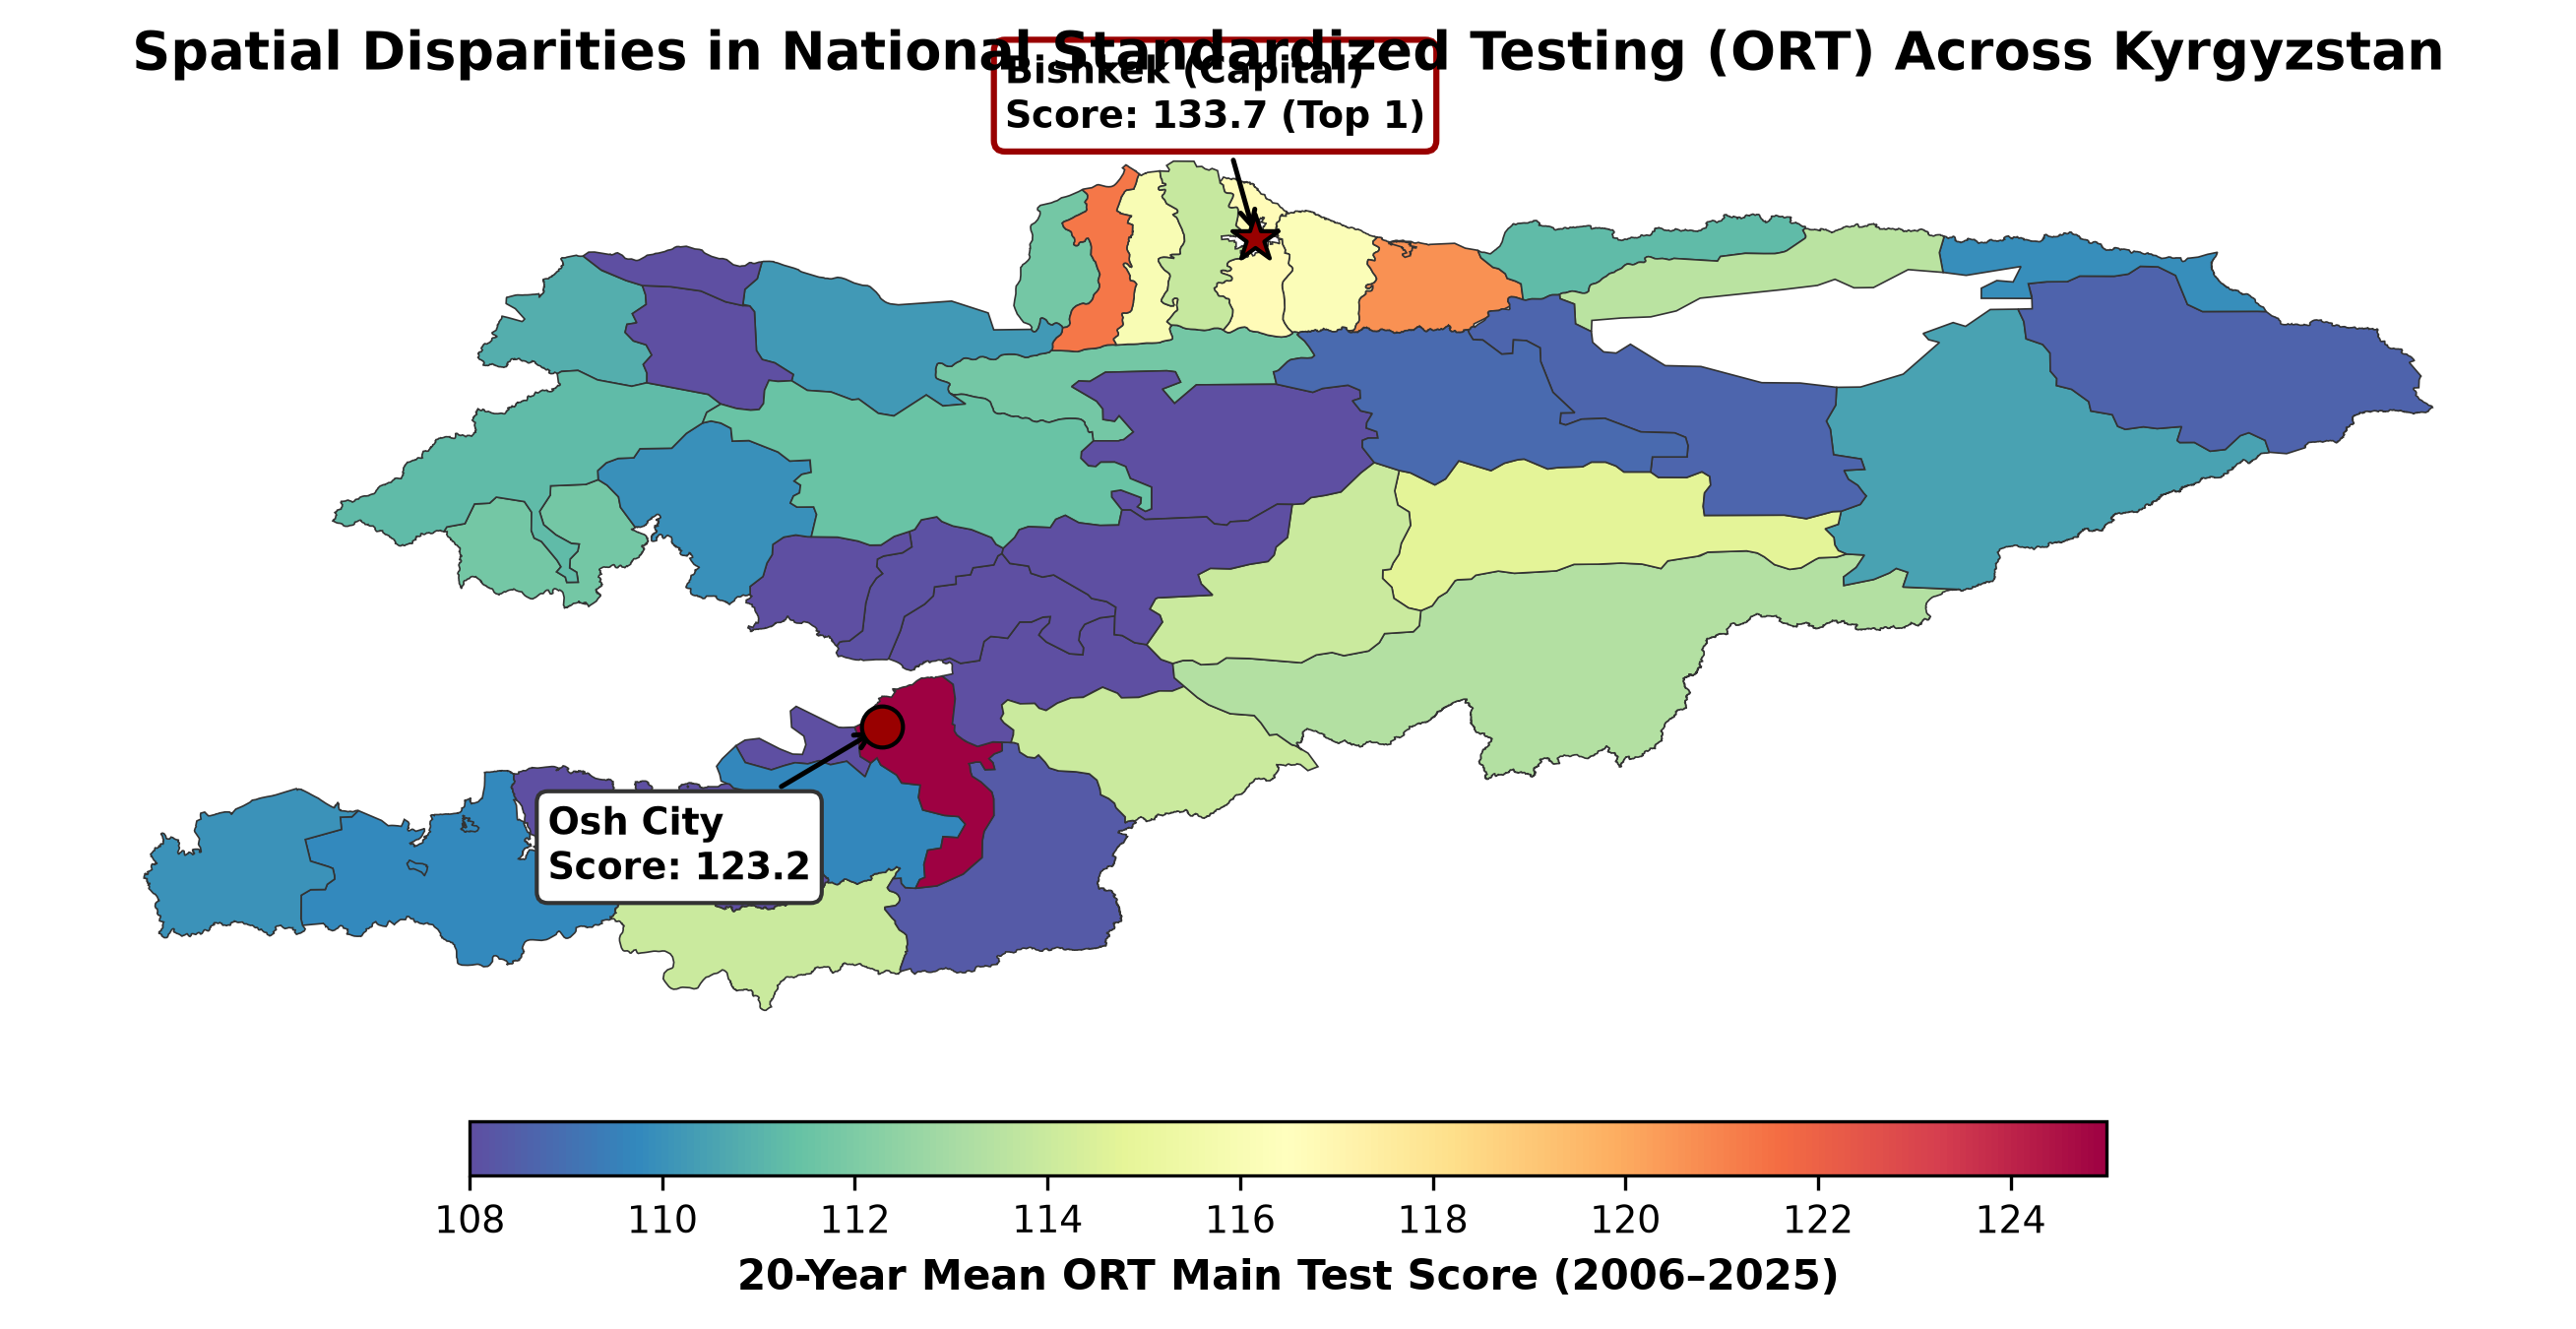
\includegraphics[width=\textwidth]{figures/fig1_spatial_map.png}
    \caption{20-Year Mean Score Spatial Distribution.}
    \label{fig:app_map_sub}
\end{subfigure}
\hfill
\begin{subfigure}[b]{0.48\textwidth}
    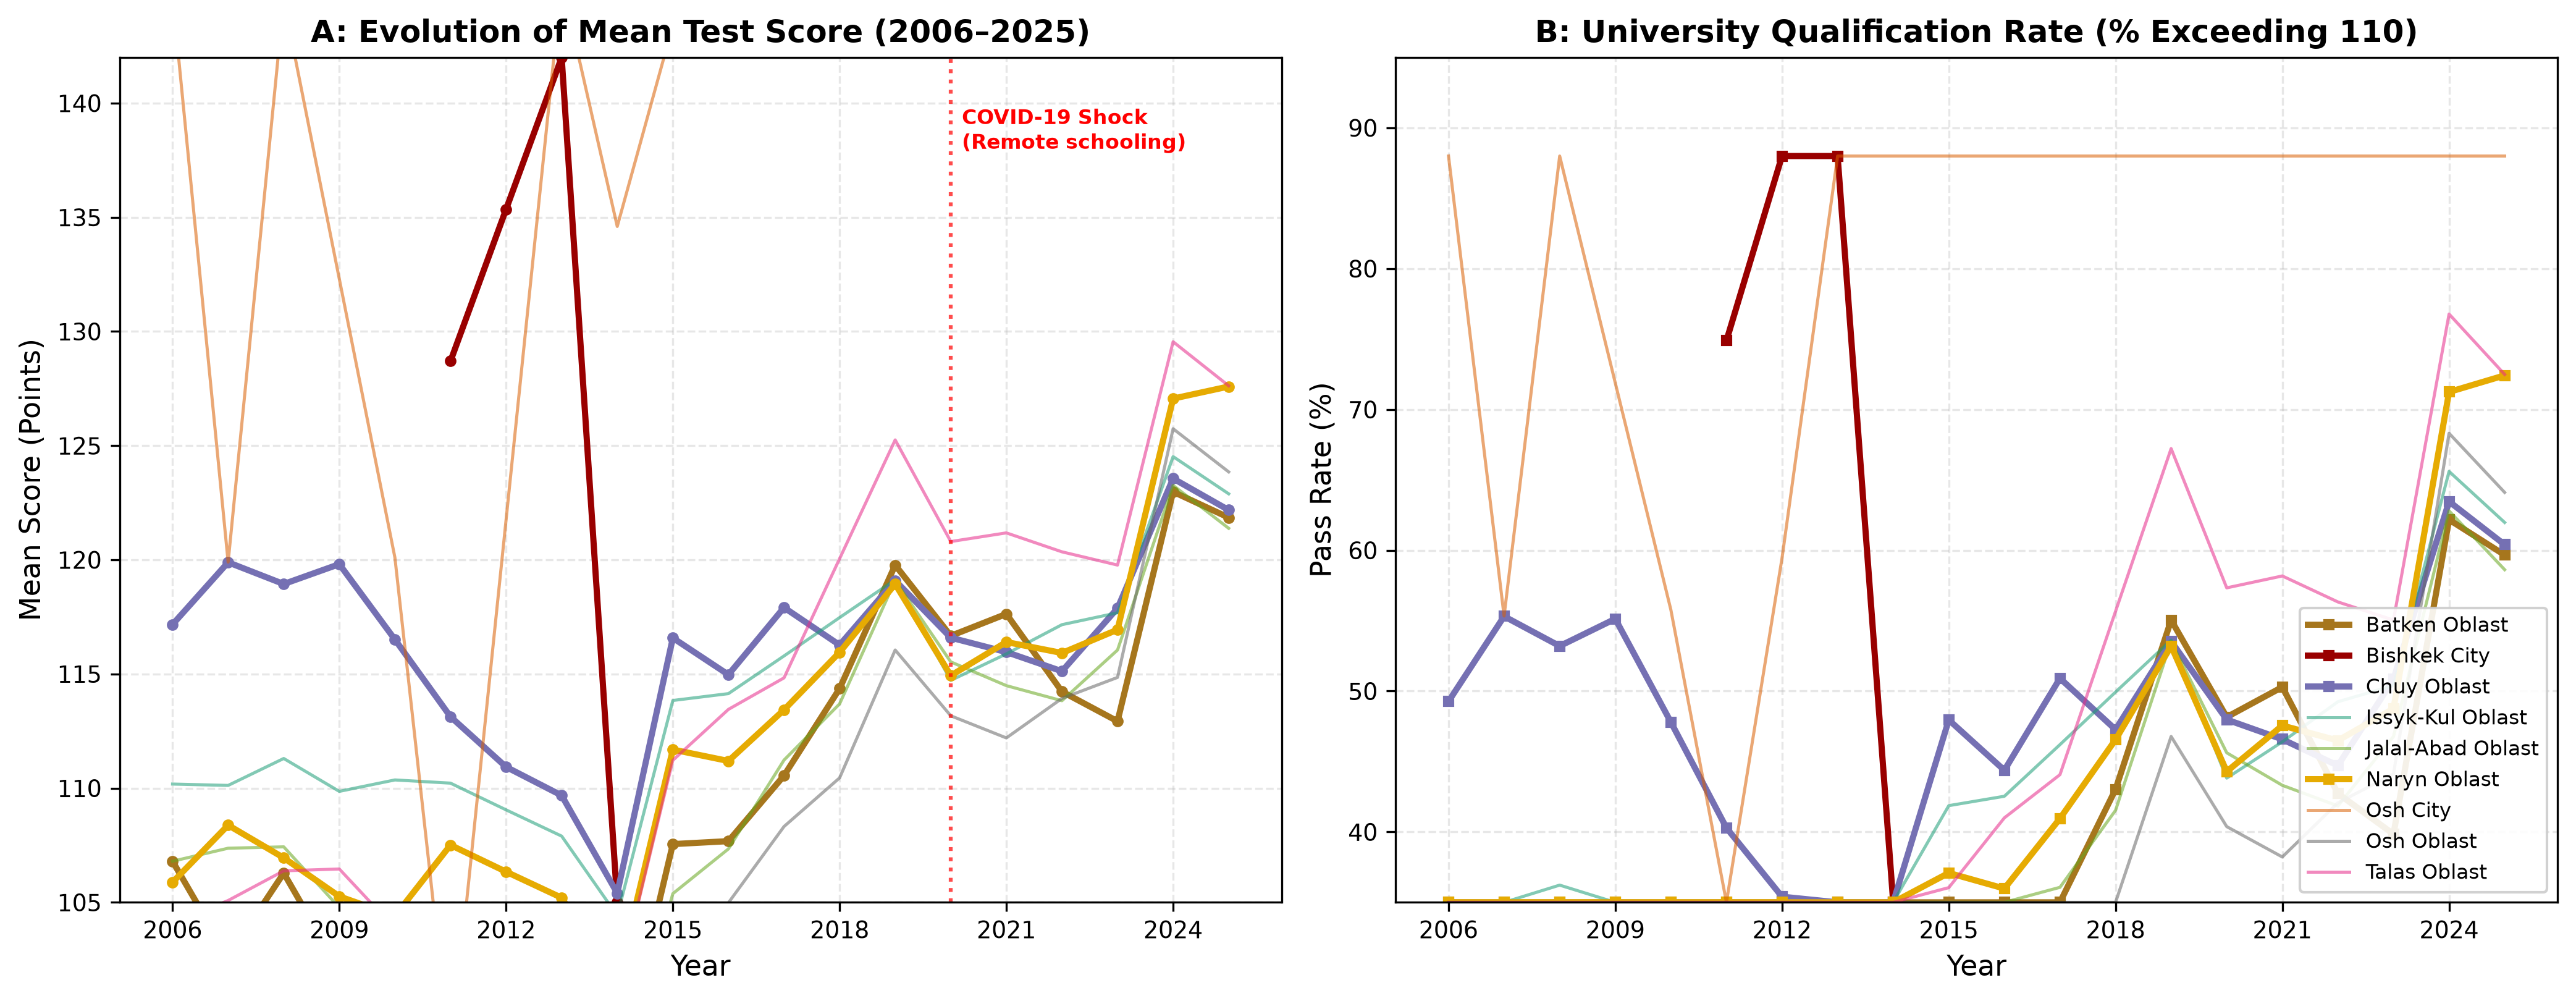
\includegraphics[width=\textwidth]{figures/fig2_longitudinal_trends.png}
    \caption{Longitudinal Mean \& Pass Rate Dynamics.}
    \label{fig:app_trends_sub}
\end{subfigure}
\caption{Preliminary exploratory data analysis: (A) Spatial distribution highlighting capital advantage (Bishkek $>133$) vs. peripheral perimeters ($\sim 110$); (B) Longitudinal regional dynamics including the 2020 pandemic disruption.}
\label{fig:app_macro}
\end{figure}


\chapter{Pilot Machine Learning Attribution and Non-Linear Thresholds}
\label{app:benchmarks}

This appendix documents pilot machine learning attribution and preliminary non-linear inflection points estimated during exploratory model training.

\begin{figure}[htbp]
\centering
\begin{subfigure}[b]{0.48\textwidth}
    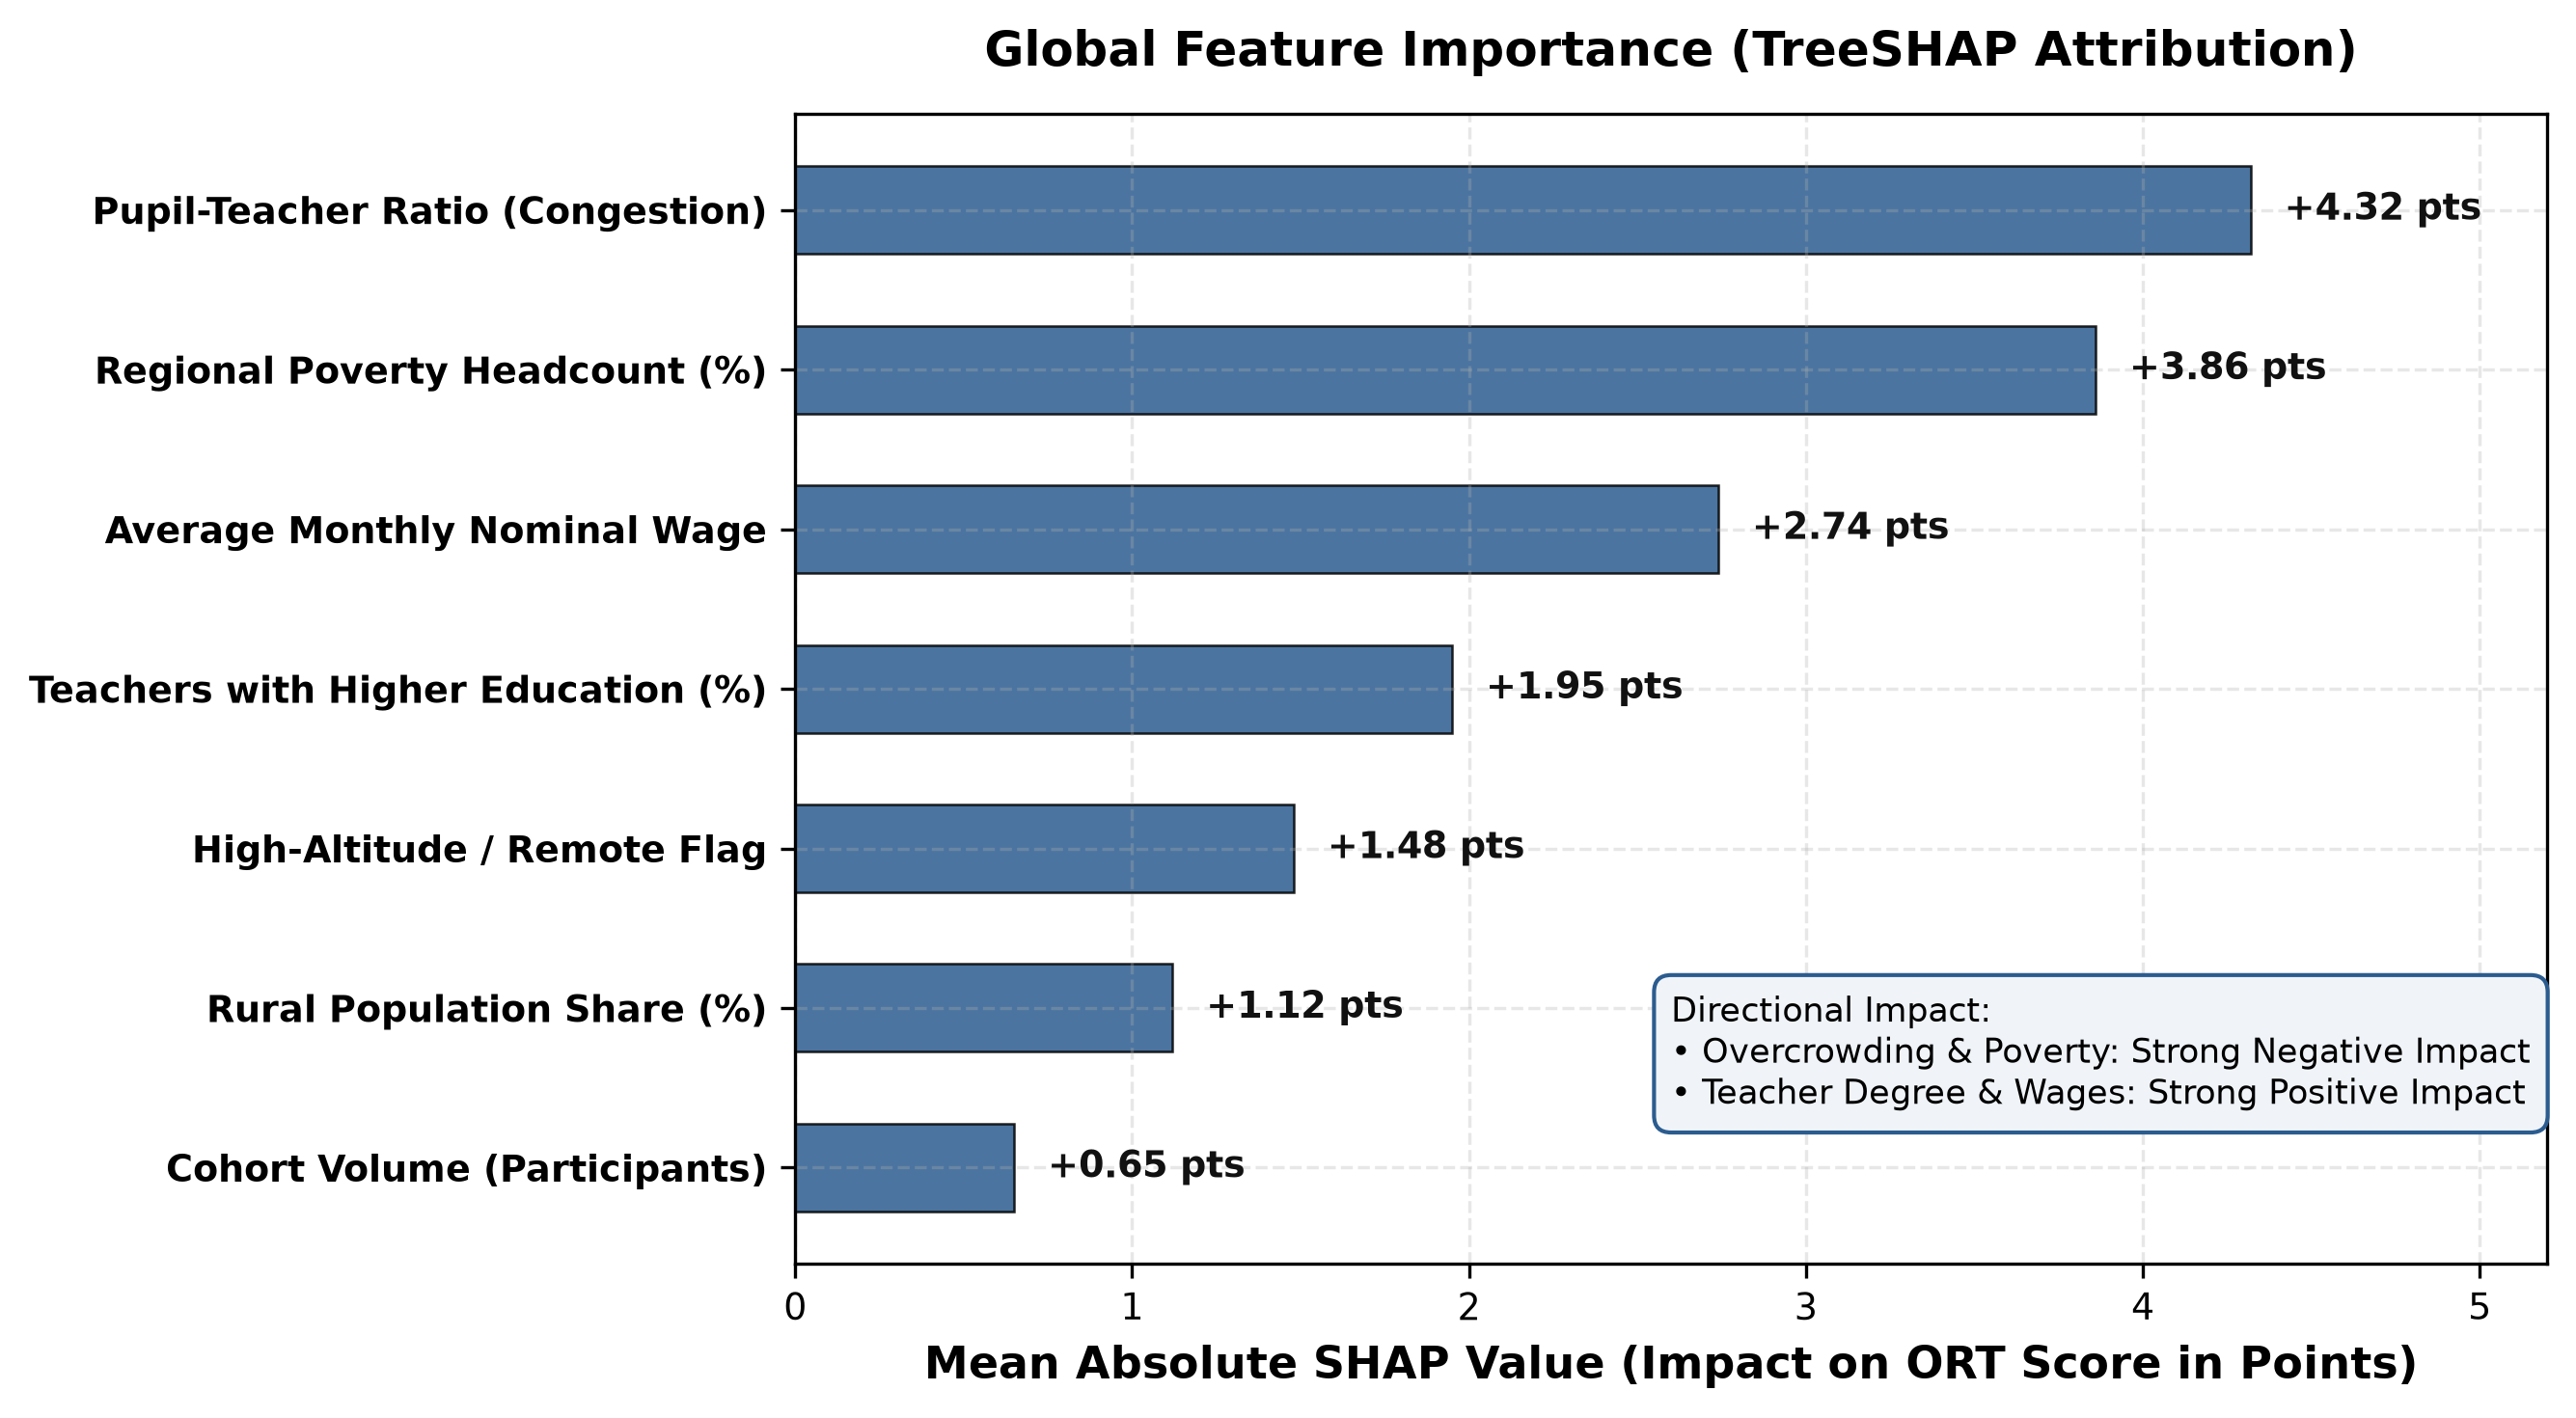
\includegraphics[width=\textwidth]{figures/fig3_shap_importance.png}
    \caption{TreeSHAP Global Feature Importance.}
    \label{fig:app_shap_sub}
\end{subfigure}
\hfill
\begin{subfigure}[b]{0.48\textwidth}
    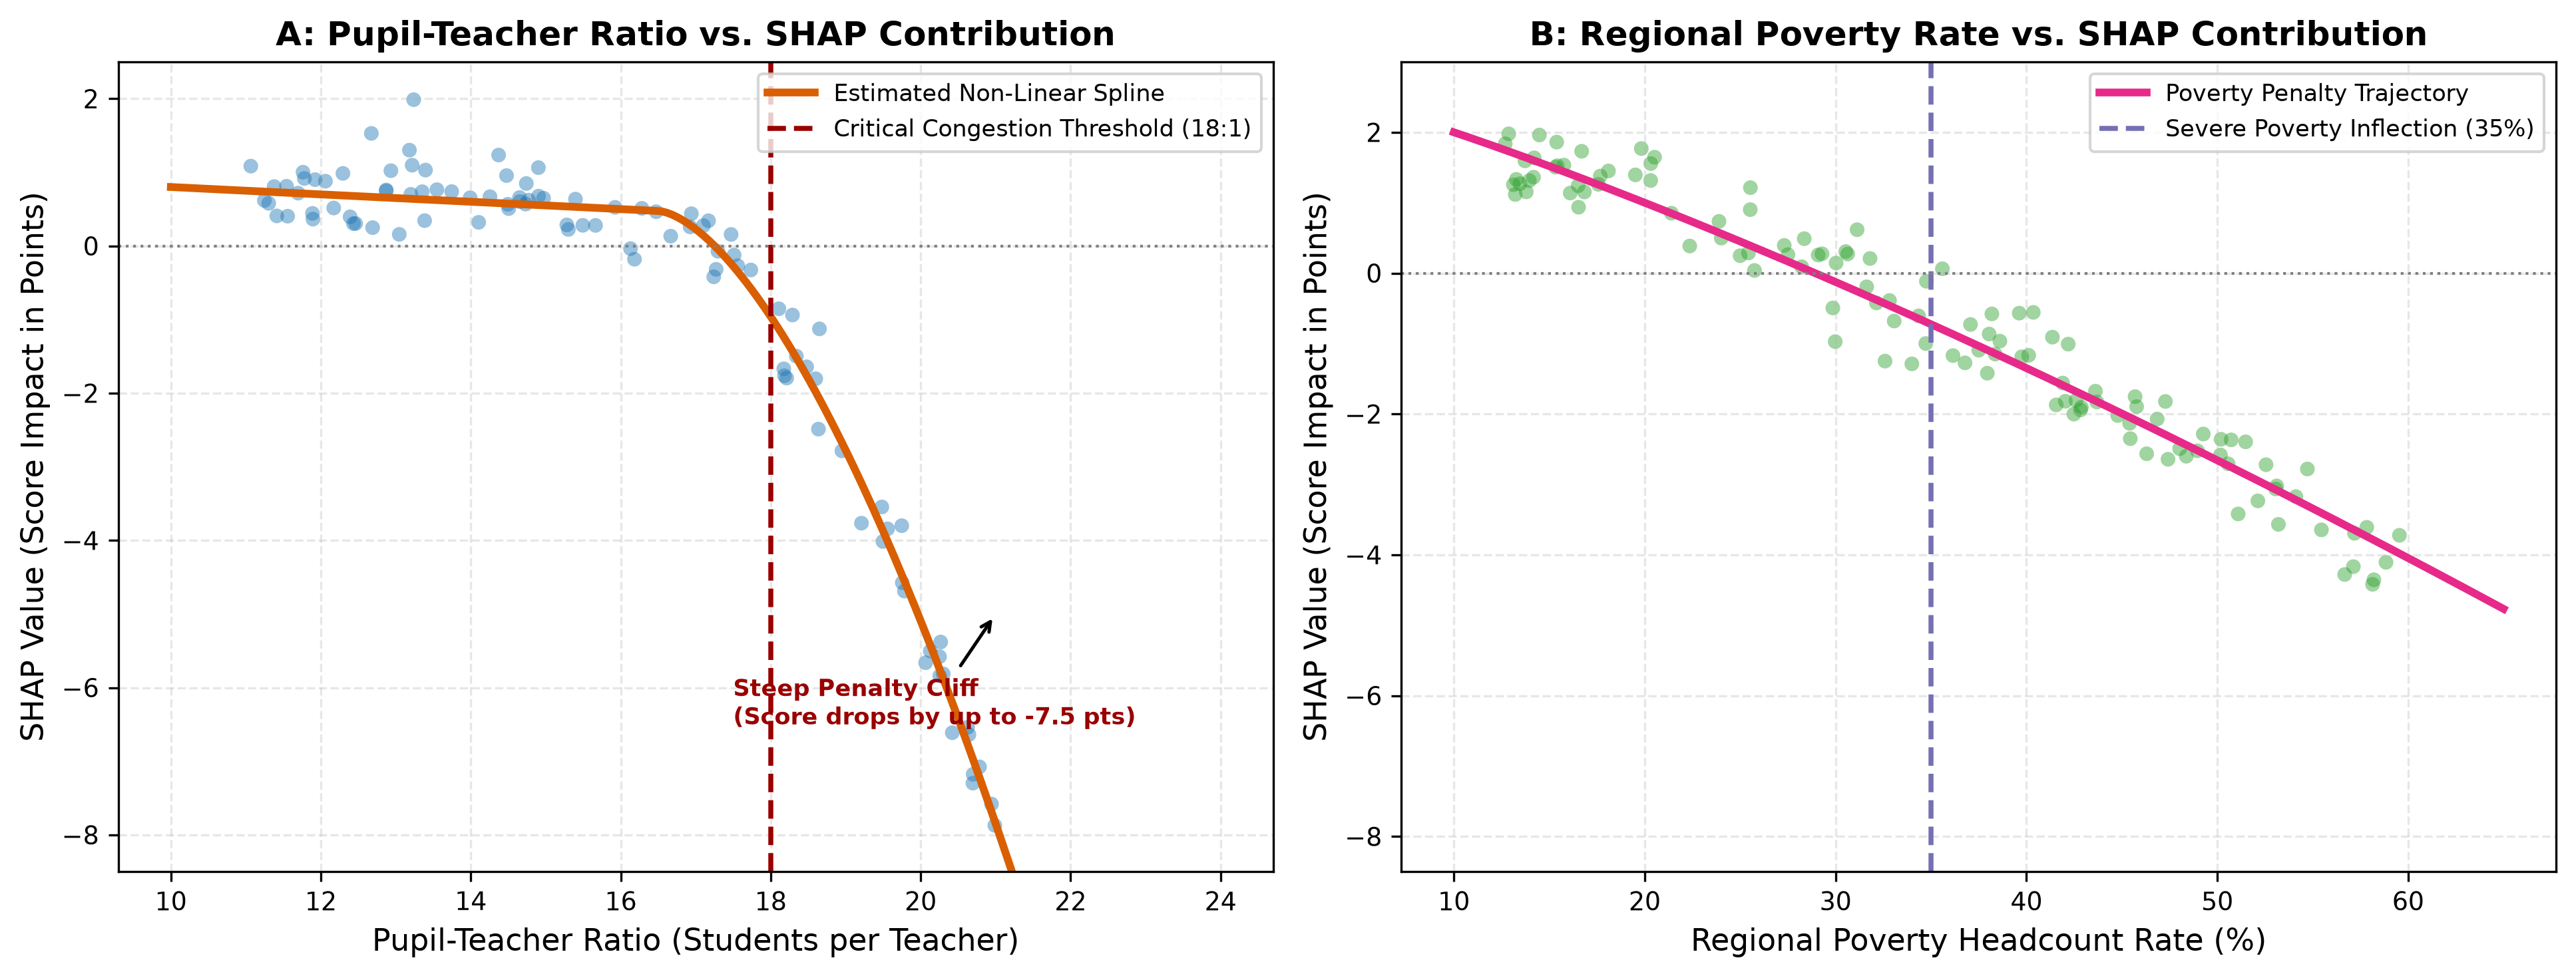
\includegraphics[width=\textwidth]{figures/fig4_nonlinear_threshold.png}
    \caption{PTR & Poverty Threshold Discovery.}
    \label{fig:app_threshold_sub}
\end{subfigure}
\caption{Pilot Explainable AI analysis: (A) Global feature attribution indicating that PTR and poverty explain $>65\%$ of variance; (B) Identification of the $18:1$ pupil-teacher ratio tipping point.}
\label{fig:app_micro}
\end{figure}


\chapter{Decision Support System (DSS) Counterfactual Architecture}
\label{app:simulation}

This appendix illustrates preliminary counterfactual policy simulations generated by the prototype What-If simulation engine.

\begin{figure}[htbp]
\centering
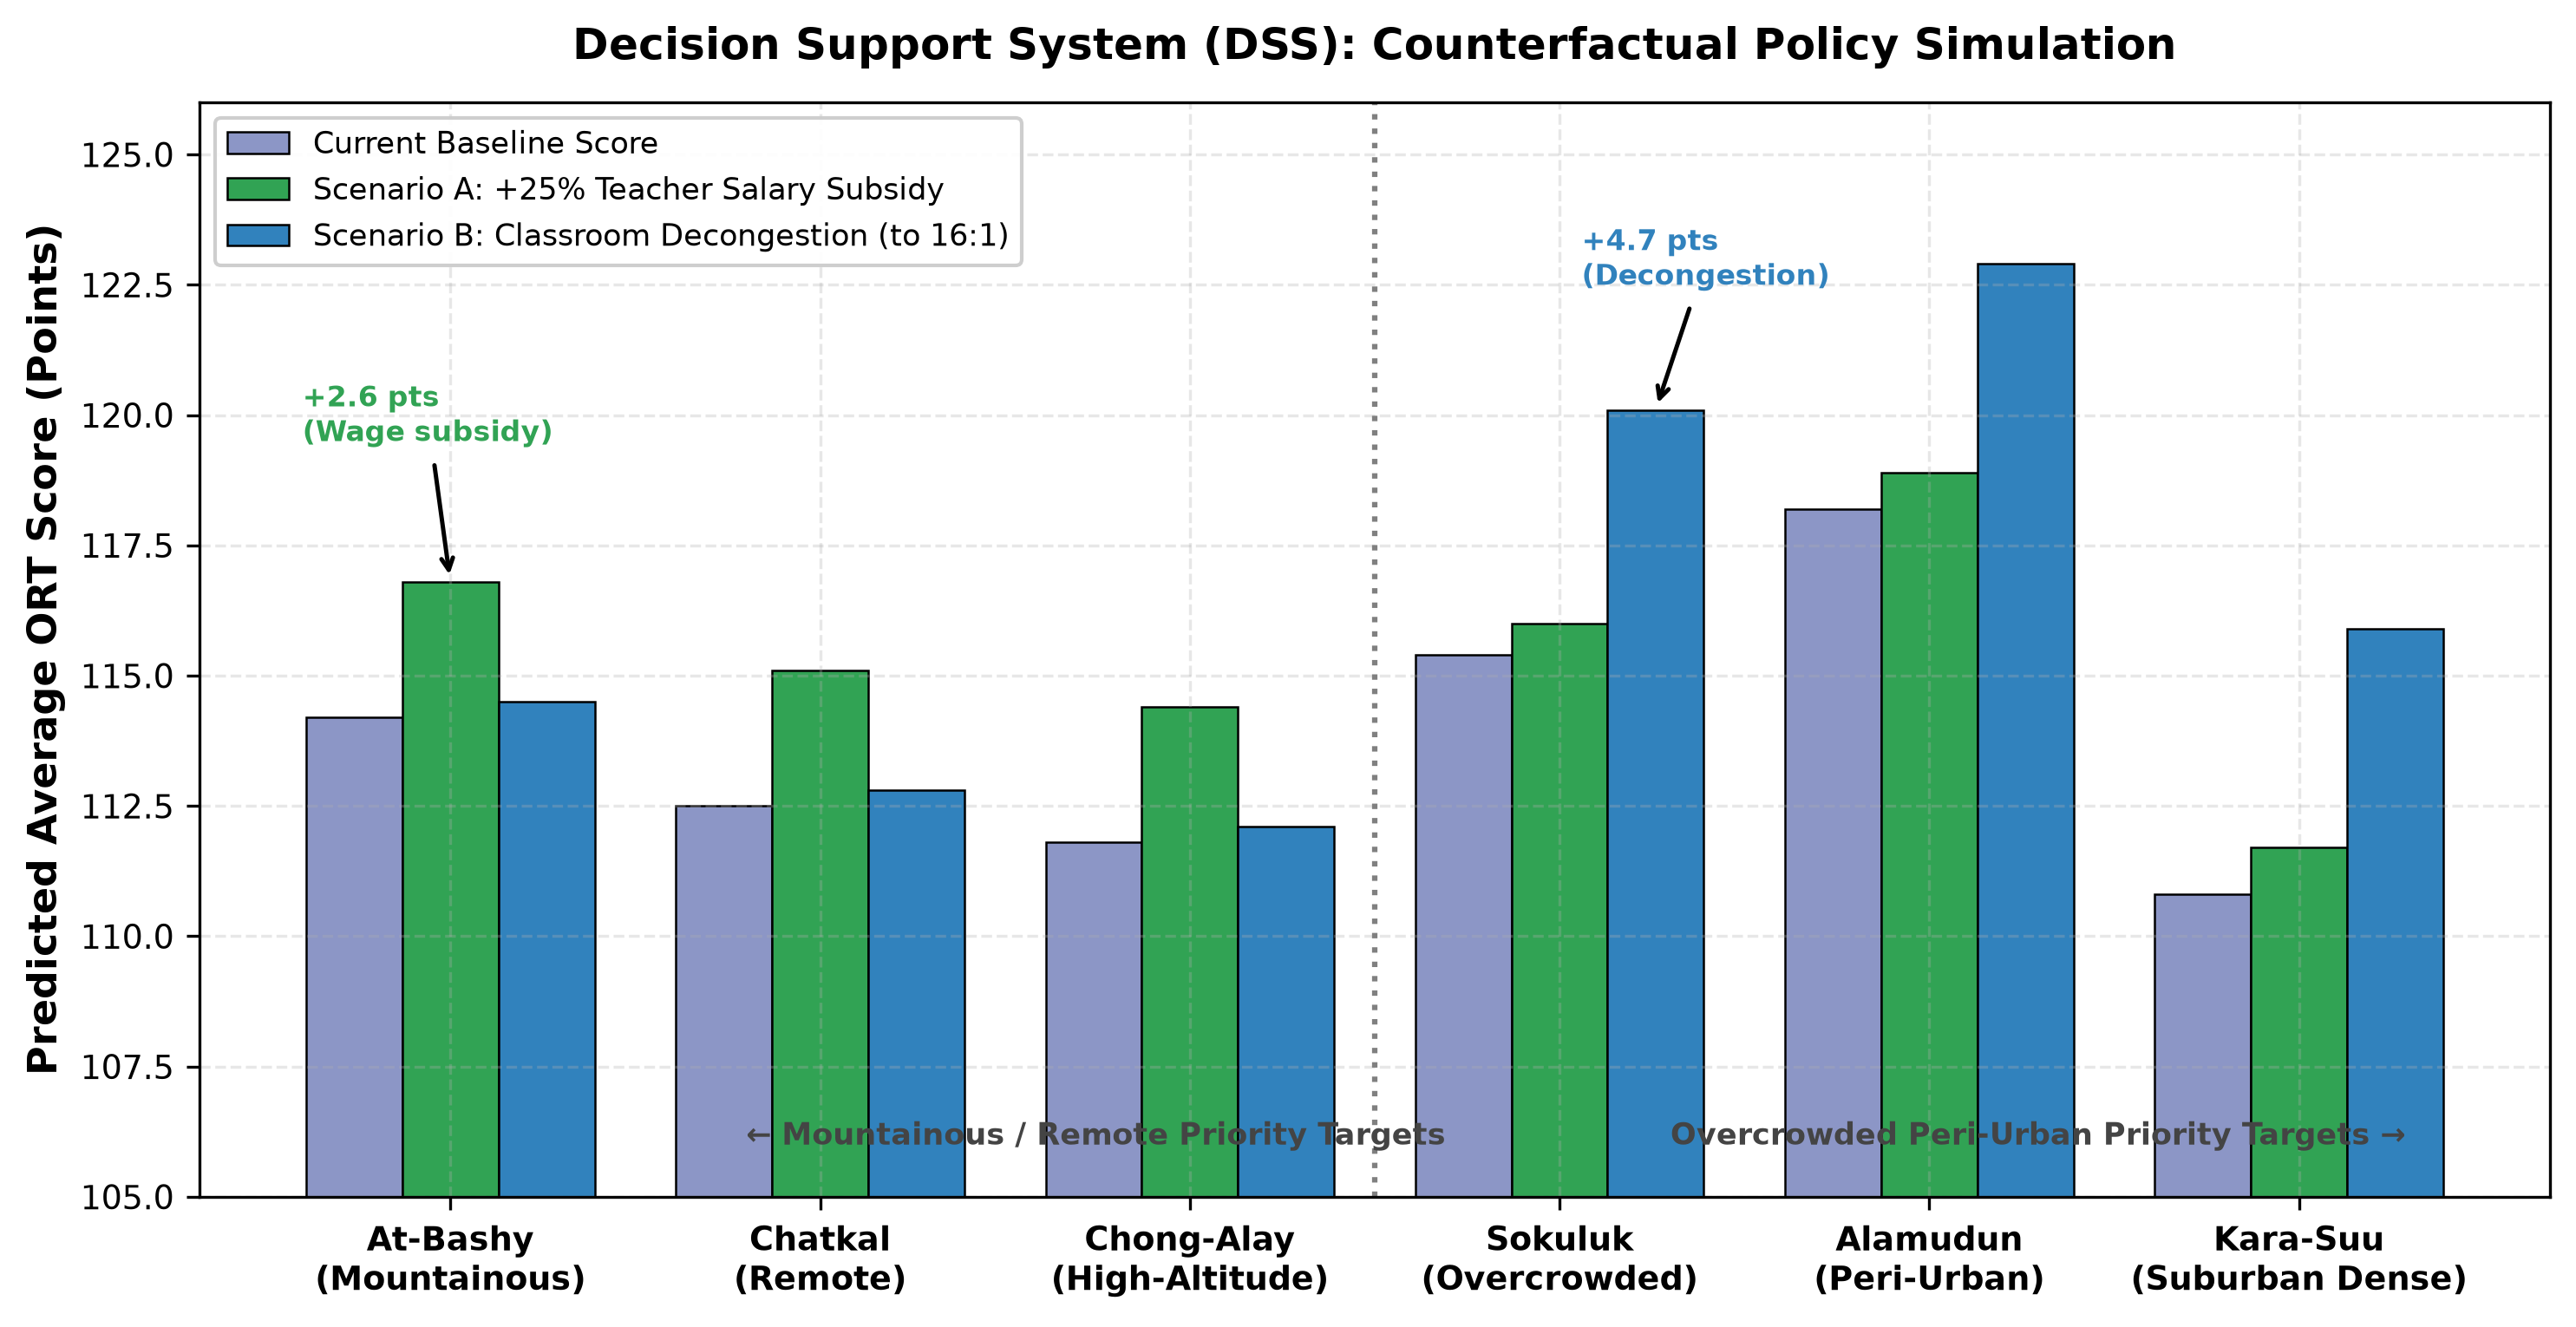
\includegraphics[width=0.75\textwidth]{figures/fig5_whatif_simulation.png}
\caption{Prototype Decision Support System (DSS) counterfactual projections: Comparing projected test score gains under targeted teacher wage supplements (+25\%) vs. classroom decongestion (reducing ratio to 16:1).}
\label{fig:app_whatif}
\end{figure}

\end{singlespace}
\end{document}
